\section{WERYFIKACJA PRACY PROGRAMU}
\label{testSection}

\subsection{Testy jednostkowe}

Działanie wszystkich funkcji wchodzących w skład bardziej skomplikowanej logiki
biznesowej programu, zawartej w module \verb|algorithms| zostało zweryfikowane
testami jednostkowymi. Wynik wykonania testów jednostkowych można zobaczyć na
listingu \ref{cargoTestListing}.

\lstinputlisting[
    float=h!,
    basicstyle=\ttfamily\small,
    frame=tb,
    label={cargoTestListing},
    caption={Wykonanie testów jednostkowych}
]{./code/cargoTest.txt}

Działanie testów jednostkowych można opisać następująco:

\begin{itemize}

    \item \verb|mermaid_diagram_generation::tests::works| - test sprawdza
        poprawność działania algorytmu generującego diagram ER w składni
        \verb|mermaid.js|. Do implementacji podawana jest przykładowa struktura
        tabel. Sprawdzane jest, czy wygenerowany diagram jest poprawny.

    \item \verb|sql_variable_parser::tests::parsing_test| - test sprawdza
        podstawową funkcję parsującą SQL wykorzystywaną do implementacji
        bardziej skomplikowanej funkcjonalności parsera.

    \item \verb|sql_variable_parser::tests::parsing_multiple| - test sprawdza
        poprawne działanie parsera SQL, gdy w jednym zapytaniu znajduje się
        większa ilość odwołań do zmiennych.

    \item \verb|sql_variable_parser::tests::bind_vec| - test sprawdza poprawność
        działania funkcji, która przekształca tablicę mieszającą zawierającą
        dostępne zmienne i sparsowany SQL na tablicę wartości, które powinny
        zostać wysłane do bazy danych.

    \item \verb|sql_variable_parser::tests::parsing_endpoint_info| - test
        sprawdza poprawność funkcji parsującej strukturę danych, którą należy
        wysłać do serwera w celu stworzenia nowego punktu końcowego.

    \item \verb|sql_variable_parser::tests::not_closed_panics| - test sprawdza,
        czy program zwraca błąd, gdy do funkcji parsującej SQL podane zostanie
        zapytanie z niepoprawną składnią (niedomknięta klamra).

    \item \verb|endpoint_execution::test::it_works| - test sprawdza podstawowe
        działanie modułu wykonującego drzewo zapytań SQL. Do implementacji
        podawane jest drzewo składające się z jednego liścia. Sprawdzane jest,
        czy zapytanie umieszczone w liściu zostało wykonane.
        
    \item \verb|endpoint_execution::test::request_variables_work| - test
        sprawdza poprawne działanie, gdy drzewo zapytań SQL zawiera zapytanie z
        odniesieniem do zmiennej pochodzącej z zapytania HTTP. Sprawdzane jest,
        czy do bazy danych wysyłane jest poprawne zapytanie SQL i poprawne
        zmienne.

    \item \verb|endpoint_execution::test::super_variables_work| - test sprawdza
        poprawne działanie, gdy drzewo zapytań SQL zawiera zapytanie z
        odniesieniem do zmiennej pochodzącej z zapytania nadrzędnego. Do modułu
        podawane jest drzewo z dwoma węzłami. Węzeł podrzędny odnosi się do
        zmiennej będącej wynikiem wykonania węzła nadrzędnego. Sprawdzana jest
        poprawna kolejność wysyłanych zapytań SQL oraz poprawność danych
        wysyłanych razem z zapytaniem podrzędnym.

    \item \verb|endpoint_execution::test::error_when_cant_find_req_variable| -
        test sprawdza, czy program zwróci błąd, gdy zapytanie odnosi się do
        zmiennej wysyłanej z zapytaniem HTTP, która nie istnieje.

    \item \verb|endpoint_execution::test::error_when_cant_find_super_variable| -
        test sprawdza czy program zwróci błąd, kiedy węzeł podrzędny zawiera
        odniesienie do zmiennej z węzła nadrzędnego, która nie istnieje.

    \item \verb|endpoint_execution::test::error_when_too_many_supers| - test
        sprawdza czy program zwróci błąd, gdy zmienna zawarta w drzewie zapytań
        sql odnosi się do zmiennej, która nie może istnieć, bo nazwa zmiennej
        zawiera więcej prefiksów ``\verb|super.|'', niż istnieje węzłów
        nadrzędnych. Do modułu podawane jest drzewo z dwoma węzłami. Węzeł
        podrzędny odnosi się do zmiennej z dwoma prefiksami ``\verb|super.|'',
        ale ma tylko jeden węzeł nadrzędny.

\end{itemize}

\subsection{Testy integracyjne}

Testy integracyjne zostały napisane w programie Postman. Jest to program służący
do testowania API. Testy napisane w tym programie można wyeksportować do pliku
json, który można wykonać z poziomu powłoki tekstowej za pomocą programu
newman. Pozwala to na automatyczne wykonywanie testów.

Wykonanie testów integracyjnych widać na listingu \ref{postmanTestExec}.

{
    \small
    \singlespacing
    \lstinputlisting[
        frame=tb,
        label={postmanTestExec},
        caption={Wykonanie testów integracyjnych za pomocą programu newman}]
    {./code/newmanIntegration.txt}
}


\FloatBarrier

Wykonanie testów integracyjnych powinno odbywać się po uruchomieniu aplikacji
backend po raz pierwszy z pustą bazą danych. Stan aplikacji zostaje zachowany
podczas całego działania testów integracyjnych. Działanie to można opisać
następująco:

\begin{enumerate}

    \item Login admin - test sprawdza, czy możliwe jest poprawne zalogowanie do
        konta administratora. Token administratora jest zapisywany i korzystają
        z niego pozostałe testy.

    \item Create users - test wysyła do serwera polecenie stworzenia
        użytkowników, sprawdza czy odpowiedź jest poprawna.

    \item Create table form - test wysyła do serwera polecenie stworzenia
        tabeli. Polecenie nie zawiera zapytania SQL. Jest to wariant polecenia,
        który wysyła aplikacja frontend przy tworzeniu nowego typu danych za
        pomocą formularza.

    \item Get table info - test wysyła do serwera zapytanie o informacje o
        tabelach zawartych w bazie danych. Test sprawdza, czy odpowiedź zawiera
        dane o tabeli stworzonej w teście 3.

    \item Insert data - test wysyła do serwera polecenie dodania danych do
        tabeli. Jest to wariant polecenia, jakie wysyła aplikacja frontend przy
        dodawaniu danych za pomocą formularza.

    \item Get data - test wysyła do serwera zapytanie o informacje zawarte w
        tabeli stworzonej w teście 3. Jest to wariant zapytania, jakie wysyła
        aplikacja frontend w edytorze danych opartym o formularze. Test
        sprawdza, czy dane są takie same, jak te dodane do tabeli w teście 5.

    \item Execute query - test wysyła do serwera zapytanie HTTP z zapytaniami
        SQL. Test wysyła zapytanie tworzące nowe dane w tabeli stworzonej w
        teście 3 oraz zwracające stworzone dane. Zapytanie zostało umieszczone
        poniżej.

        \begin{verbatim}
insert into test_table_one (name, age)
    values ('Adam Nowak', 42)
    returning name, age::text
        \end{verbatim}

        Ponadto, zapytanie zawiera zapytanie SQL wykonywane przed i po wykonaniu
        drzewa zapytań. Jest to zapytanie pobierające wartości z kolumny
        \verb|name| z tabeli \verb|test_table_one|. Test sprawdza czy zapytanie
        zostało poprawnie wykonane oraz czy wartości zapytania wykonywanego
        przed i po drzewie zapytań są poprawne.

    \item Test endpoint - test wysyła do serwera zapytanie będące wariantem
        zapytania, jakie wysyła aplikacja frontend w celu przetestowania
        tworzonego punktu końcowego. Test sprawdza poprawność odesłanej przez
        serwer odpowiedzi.

    \item Create endpoint - test wysyła do serwera zapytanie będące wariantem
        zapytania, które aplikacja frontend wysyła w celu stworzenia punktu
        końcowego. Test sprawdza, czy odpowiedź od serwera ma kod HTTP 200 OK.

    \item Call endpoint as admin - test wywołuje punkt końcowy stworzony w
        teście 8. Test sprawdza, czy wysłana przez serwer odpowiedź zawiera
        poprawne dane. Test sprawdza, czy administrator może wywoływać dowolne
        punkty końcowe nawet, gdy nie ma go na liście użytkowników, którzy mają
        dostęp do punktu końcowego.

    \item Get endpoints - test wysyła do serwera zapytanie będące wariantem
        zapytania wysyłanego przez aplikację frontend w celu pobrania od serwera
        informacji o istniejących punktach końcowych. Test sprawdza, czy w
        odpowiedzi znajdują się dane o punkcie końcowym stworzonym w teście 8.

    \item Create manager user - test tworzy użytkownika należącego do grupy
        \verb|MANAGERS|. Ta grupa ma dostęp do punktu końcowego stworzonego w
        teście 8.

    \item Try call worker - test próbuje wywołać punkt końcowy przy pomocy konta
        użytkownika stworzonego w teście 2. Użytkownik nie ma uprawnień do
        wywoływania tego punktu końcowego. Test sprawdza, czy zwrócono kod HTTP
        401 oznaczający brak dostępu.

    \item Call manager - test wywołuje punkt końcowy stworzony w teście 8 przy
        użyciu konta kierownika stworzonego w teście 11. Użytkownik ma możliwość
        wywoływania punktu końcowego. Test sprawdza, czy punkt końcowy został
        wywołany.

\end{enumerate}

\subsection{Testy manualne}

Poprawne działanie najważniejszych funkcji aplikacji frontend zostało
zweryfikowane za pomocą testów manualnych. Scenariusze testów manualnych zostały
przedstawione poniżej.

\begin{enumerate}

    \item \textbf{Testowanie poprawnego działania systemu kart.}

        \begin{enumerate}

            \item \textbf{Testowanie poprawnego tworzenia nowej karty.}

                \textbf{Przebieg testu:}

                \begin{enumerate}

                    \item Wciśnięcie przycisku ``+'' po lewej stronie paska
                        kart.

                \end{enumerate}

                \textbf{Spodziewany wynik:}

                Jeśli ostatnia karta znajduje się na widoku startowym, powinna
                zostać wybrana jako aktywna. Jeśli już była aktywna, powinna
                pozostać aktywna.

                Jeśli ostatnia karta nie znajduje się na widoku startowym,
                powinna zostać stworzona nowa karta znajdująca się na widoku
                startowym. Nowa karta powinna zostać wybrana jako aktywna.

                Przebieg testu został przedstawiony na rysunku \ref{cardCreationManualTest}.

                \begin{figure}[h]
                    \centering

                    \subfloat[\centering Przed wykonaniem]
                    {{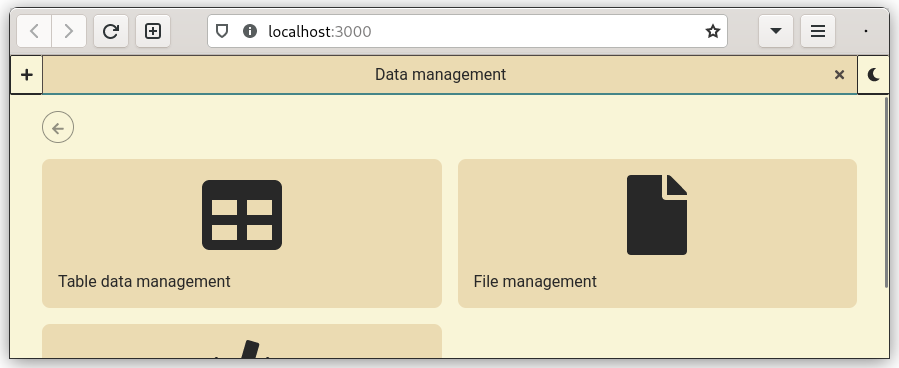
\includegraphics[width=.8\linewidth]{./img/cards/creating_cards/1_pre.png} }}

                    \subfloat[\centering Po wykonaniu]
                    {{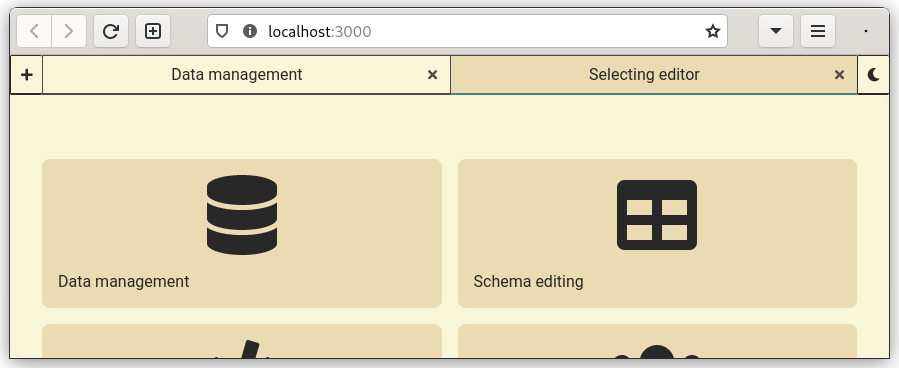
\includegraphics[width=.8\linewidth]{./img/cards/creating_cards/2_post.png} }}

                    \subfloat[\centering Przed wykonaniem, gdy ostatnia karta jest na widoku
                    startowym]
                    {{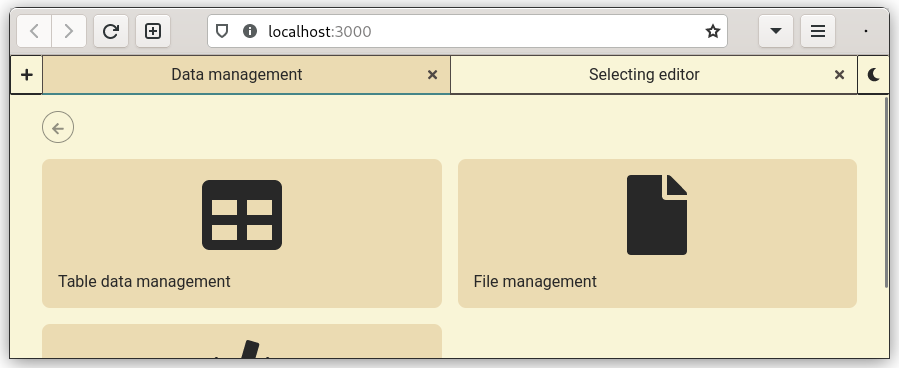
\includegraphics[width=.8\linewidth]{./img/cards/creating_cards/3_pre.png} }}

                    \subfloat[\centering Po wykonaniu, gdy ostatnia karta była na widoku startowym]
                    {{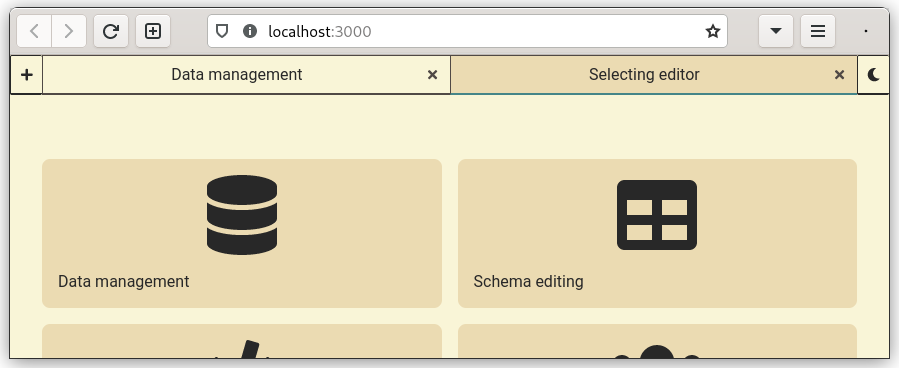
\includegraphics[width=.8\linewidth]{./img/cards/creating_cards/4_post.png} }}

                    \caption{Przebieg testu tworzenia kart}
                    \label{cardCreationManualTest}
                \end{figure}

                \FloatBarrier

            \item \textbf{Testowanie poprawnego zamykania karty.}

                \textbf{Przebieg testu:}

                \begin{enumerate}

                    \item Wciśnięcie przycisku ``x'' po prawej stronie karty,
                        lub wciśnięcie dowolnego miejsca karty środkowym
                        przyciskiem myszki.

                \end{enumerate}

                \textbf{Spodziewany wynik:}

                Jeśli karta, którą spróbowano zamknąć jest jedyną kartą i
                jest na widoku startowym, nie powinno się nic stać. Jeśli karta
                jest jedyną i nie jest na widoku startowym, w karcie powinien
                zostać otworzony widok startowy.

                Jeśli karta, którą spróbowano zamknąć nie jest jedyną kartą,
                karta powinna przestać istnieć. Dowolna sąsiednia karta do karty
                zamkniętej powinna zostać wybrana jako aktywna.

                Przebieg testu został przedstawiony na rysunku \ref{cardClosingManualTest}.

                \begin{figure}[h]
                    \centering

                    \subfloat[\centering Przed wykonaniem, gdy istnieje jedna karta]
                    {{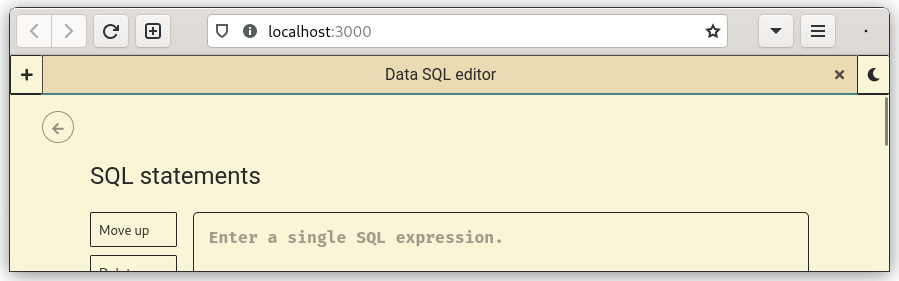
\includegraphics[width=.8\linewidth]{./img/cards/closing_cards/1_pre.png} }}

                    \subfloat[\centering Po wykonaniu, gdy istniała jedna karta]
                    {{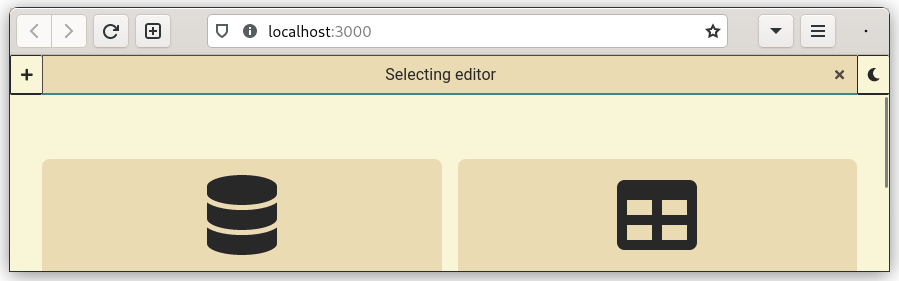
\includegraphics[width=.8\linewidth]{./img/cards/closing_cards/2_post.png} }}

                    \subfloat[\centering Przed wykonaniem, gdy istnieje wiele kart]
                    {{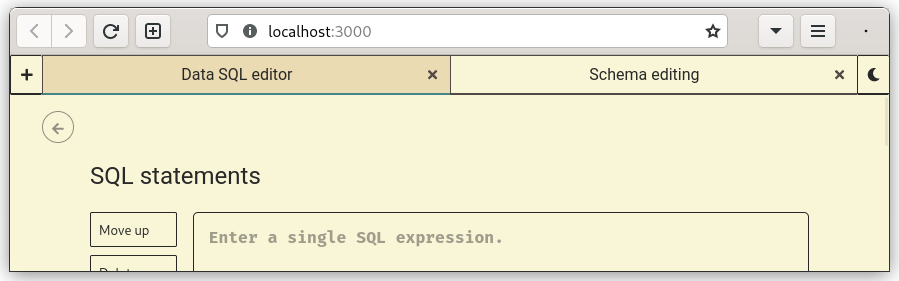
\includegraphics[width=.8\linewidth]{./img/cards/closing_cards/3_pre.png} }}

                    \subfloat[\centering Po wykonaniu, gdy istniało wiele kart]
                    {{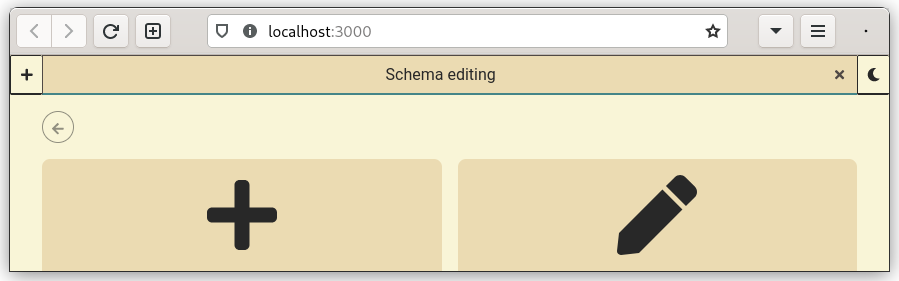
\includegraphics[width=.8\linewidth]{./img/cards/closing_cards/4_post.png} }}

                    \caption{Przebieg testu zamykania kart}
                    \label{cardClosingManualTest}
                \end{figure}

                \FloatBarrier

            \item \textbf{Testowanie poprawnego zachowania stanu w karcie.}

                \textbf{Przebieg testu:}

                \begin{enumerate}

                    \item Otworzenie w dowolnej karcie komponentu zawierającego
                        stan (na przykład pole tekstowe).

                    \item Zmiana stanu komponentu (na przykład wpisanie dowolnego
                        tekstu do pola tekstowego).

                    \item Przełączenie aktywnej karty na dowolną inną kartę.

                    \item Przełączenie aktywnej karty na kartę otwartą w kroku
                        i.

                \end{enumerate}

                \textbf{Spodziewany wynik:}

                Stan komponentu po ponownym otwarciu karty powinien być
                identyczny do stanu przed pierwszym przełączeniem aktywnej
                karty.

                Przebieg testu został przedstawiony na rysunku \ref{stateRetentionManualTest}.

                \begin{figure}[h]
                    \centering

                    \subfloat[\centering Przed zmianą karty]
                    {{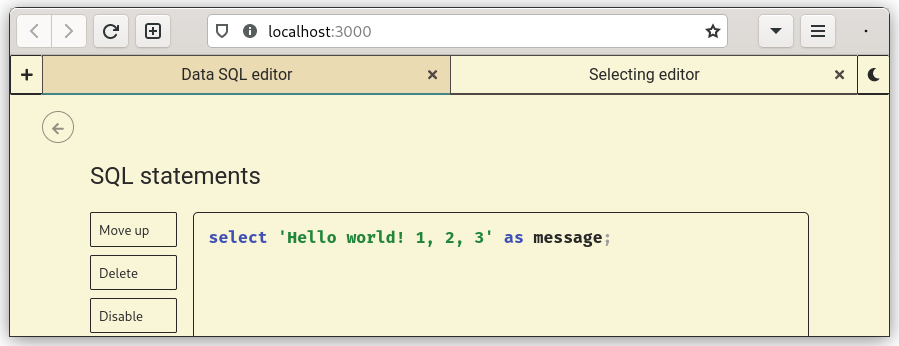
\includegraphics[width=.8\linewidth]{./img/state_retention/1.png} }}

                    \subfloat[\centering Po zmianie karty]
                    {{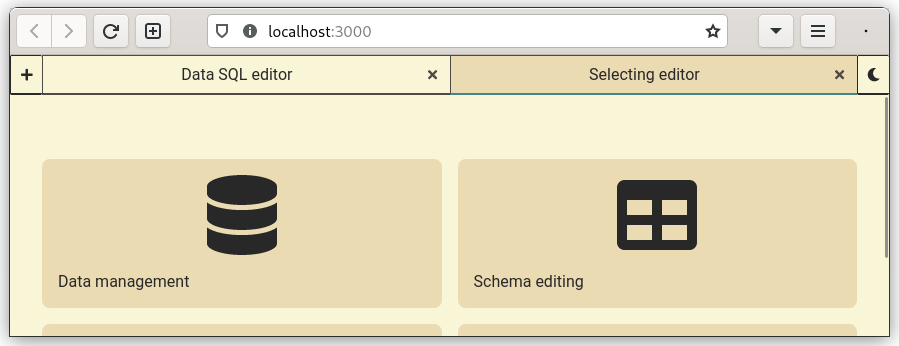
\includegraphics[width=.8\linewidth]{./img/state_retention/2.png} }}

                    \subfloat[\centering Po ponownym otwarciu karty z rysunku (a)]
                    {{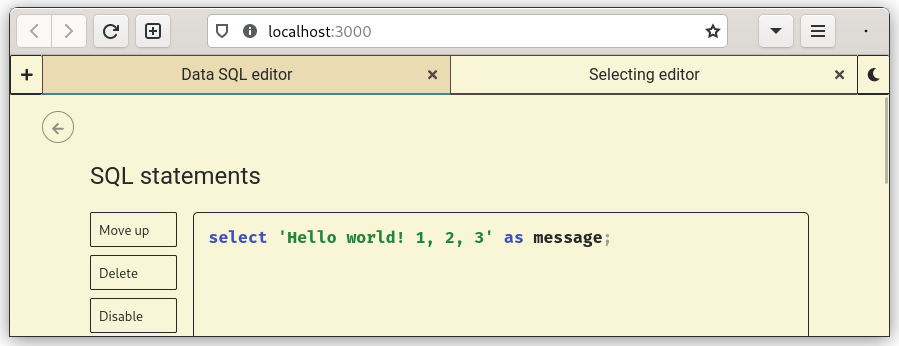
\includegraphics[width=.8\linewidth]{./img/state_retention/3.png} }}

                    \caption{Przebieg testu zachowania stanu w karcie}
                    \label{stateRetentionManualTest}
                \end{figure}

                \FloatBarrier

        \end{enumerate}

    \item \textbf{Testowanie poprawnego działania edytora zapytań SQL
        wykonywanych natychmiast.}

        \begin{enumerate}

            \item \textbf{Testowanie poprawnego tworzenia nowego zapytania.}

                \textbf{Przebieg testu:}

                \begin{enumerate}

                    \item Wciśnięcie przycisku ``New block'' pod ostatnim
                        polem tekstowym z zapytaniem SQL.

                \end{enumerate}

                \textbf{Spodziewany wynik:}

                Pod ostatnim edytorem zapytania SQL pojawi się nowy edytor
                zapytania SQL.

                Przebieg testu został przedstawiony na rysunku \ref{newBlockCreationManualTest}.

                \begin{figure}[h]
                    \centering

                    \subfloat[\centering Przed wykonaniem]
                    {{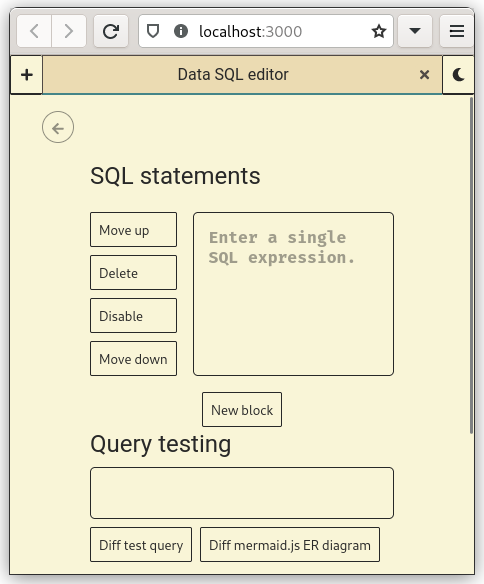
\includegraphics[width=.45\linewidth]{./img/sql_editor/new_block/1.png} }}
                    \medspace
                    \subfloat[\centering Po wykonaniu]
                    {{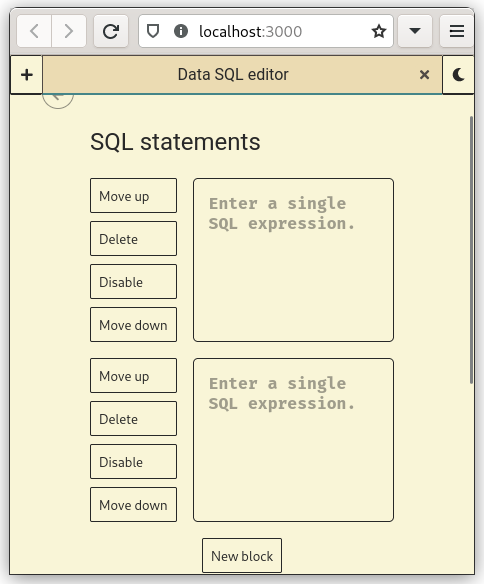
\includegraphics[width=.45\linewidth]{./img/sql_editor/new_block/2.png} }}

                    \caption{Przebieg testu tworzenia nowego zapytania}
                    \label{newBlockCreationManualTest}
                \end{figure}

                \FloatBarrier

            \item \textbf{Testowanie poprawnego usuwania zapytania SQL.}

                \textbf{Przebieg testu:}

                \begin{enumerate}

                    \item Wciśnięcie przycisku ``Delete'' po lewej stronie pola
                        tekstowego z zapytaniem SQL.

                \end{enumerate}

                \textbf{Spodziewany wynik:}

                Jeśli edytor jest jedynym edytorem, treść zapytania SQL zostanie
                usunięta.

                Jeśli edytor nie jest jedynym edytorem, zostanie usunięty z
                listy edytorów.

                Przebieg testu został przedstawiony na rysunku \ref{blockDeletionManualTest}.

                \begin{figure}[h]
                    \centering

                    \subfloat[\centering Przed wykonaniem, gdy jest więcej, niż jedno zapytanie]
                    {{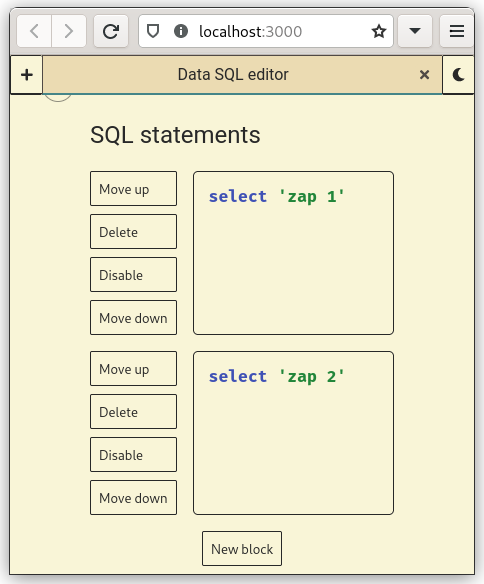
\includegraphics[width=.45\linewidth]{./img/sql_editor/deleting_block/1.png} }}
                    \medspace
                    \subfloat[\centering Po wykonaniu, gdy było więcej, niż jedno zapytanie]
                    {{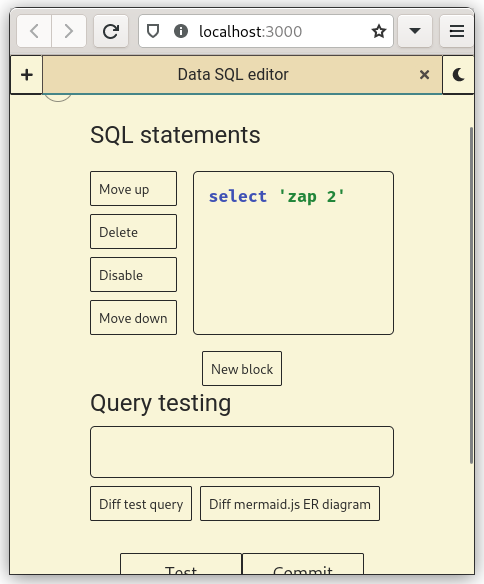
\includegraphics[width=.45\linewidth]{./img/sql_editor/deleting_block/2.png} }}

                    \subfloat[\centering Przed wykonaniem, jest tylko jedno zapytanie]
                    {{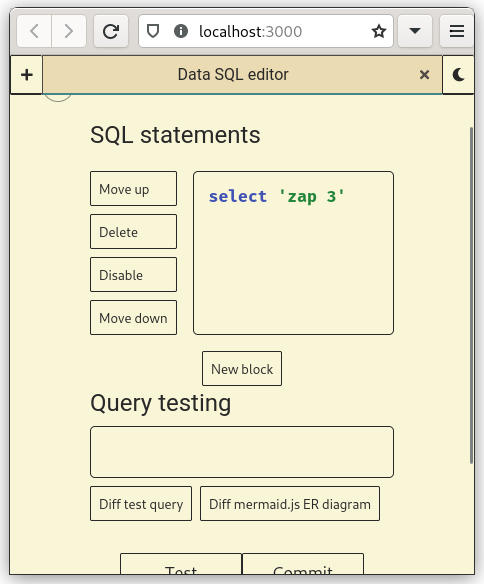
\includegraphics[width=.45\linewidth]{./img/sql_editor/deleting_block/3.png} }}
                    \medspace
                    \subfloat[\centering Po wykonaniu, gdy było tylko jedno zapytanie]
                    {{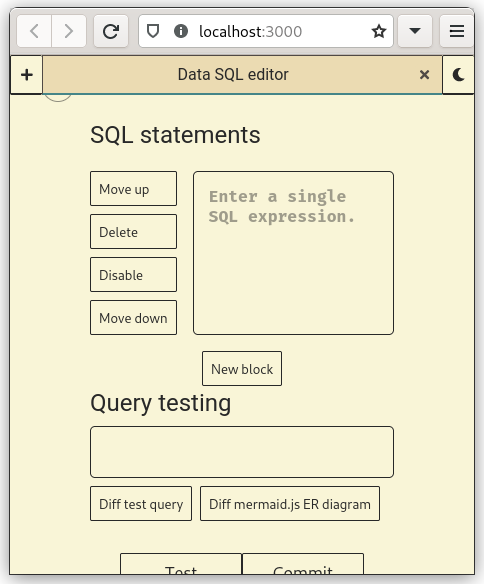
\includegraphics[width=.45\linewidth]{./img/sql_editor/deleting_block/4.png} }}

                    \caption{Przebieg testu usuwania zapytania}
                    \label{blockDeletionManualTest}
                \end{figure}

                \FloatBarrier

            \item \textbf{Testowanie poprawnego wyłączania zapytania SQL.}

                \textbf{Przebieg testu:}

                \begin{enumerate}

                    \item Wciśnięcie przycisku ``Disable'' po lewej stronie pola
                        tekstowego z zapytaniem SQL.

                    \item Wciśnięcie przycisku ``Enable'' po lewej stronie pola
                        tekstowego z zapytaniem SQL.

                \end{enumerate}

                \textbf{Spodziewany wynik:}

                Po wciśnięciu przycisku ``Disable'', tło zostanie przyciemnione w
                trybie jasnym lub rozjaśnione w trybie ciemnym. Całe pole
                tekstowe stanie się przezroczyste. Pisanie w polu tekstowym nie
                będzie możliwe.

                Po wciśnięciu przycisku ``Enable'', działanie przycisku
                ``Disable'' zostanie odwrócone.

                Przebieg testu został przedstawiony na rysunku \ref{blockDisablingManualTest}.

                \begin{figure}[h]
                    \centering

                    \subfloat[\centering Przed wykonaniem]
                    {{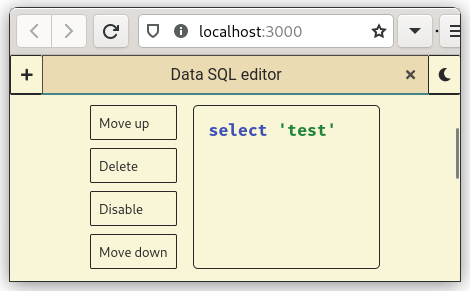
\includegraphics[width=.45\linewidth]{./img/sql_editor/disabling_block/1.png} }}
                    \medspace
                    \subfloat[\centering Po wciśnięciu ``Disable'']
                    {{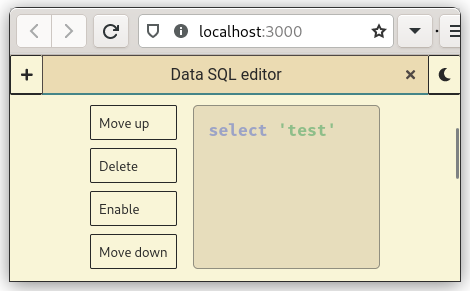
\includegraphics[width=.45\linewidth]{./img/sql_editor/disabling_block/2.png} }}

                    \subfloat[\centering Po wciśnięciu ``Enable'']
                    {{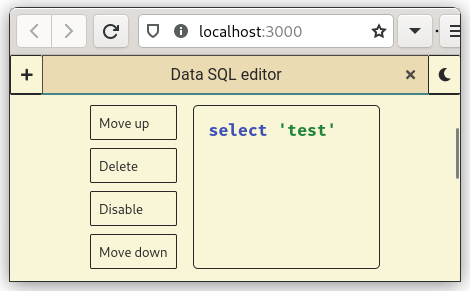
\includegraphics[width=.45\linewidth]{./img/sql_editor/disabling_block/3.png} }}

                    \caption{Przebieg testu wyłączania zapytania}
                    \label{blockDisablingManualTest}
                \end{figure}

                \FloatBarrier

        \end{enumerate}

    \item \textbf{Testowanie poprawnego działania edytora punktów końcowych.}

        \begin{enumerate}

            \item \textbf{Testowanie poprawnego tworzenia nowego drzewa zapytań SQL.}

                \textbf{Przebieg testu:}

                \begin{enumerate}

                    \item Wciśnięcie przycisku ``New independent query'' pod
                        ostatnim polem tekstowym z zapytaniem SQL.

                \end{enumerate}

                \textbf{Spodziewany wynik:}

                Pod ostatnim zapytaniem zostanie stworzone nowe zapytanie będące
                korzeniem nowego drzewa niezależnego od pozostałych zapytań.

                Przebieg testu został przedstawiony na rysunku \ref{creatingNewTreeManualTest}.

                \begin{figure}[h]
                    \centering

                    \subfloat[\centering Przed wykonaniem]
                    {{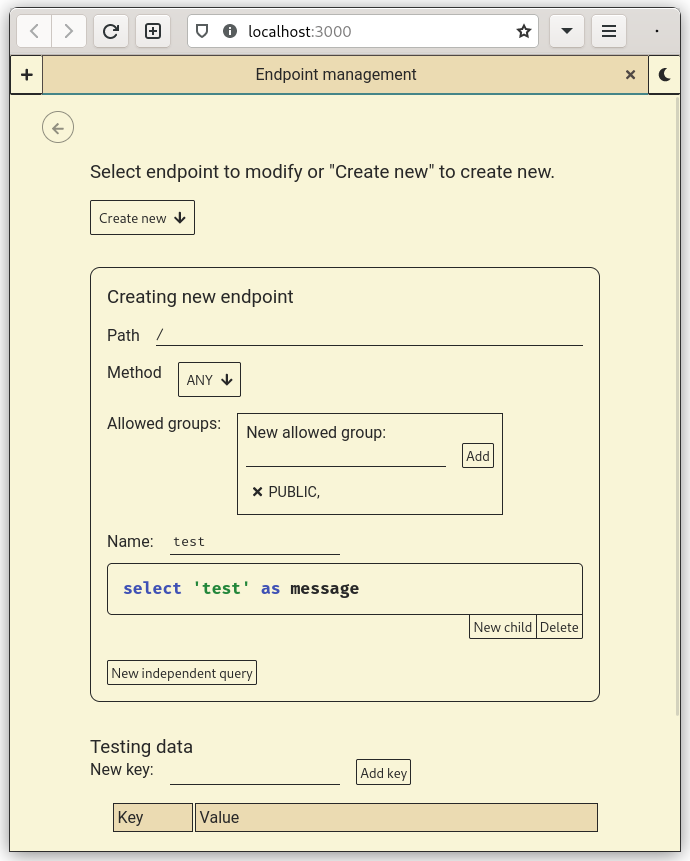
\includegraphics[width=.60\linewidth]{./img/endpoint_editor/creating_new/1.png} }}

                    \subfloat[\centering Po wykonaniu]
                    {{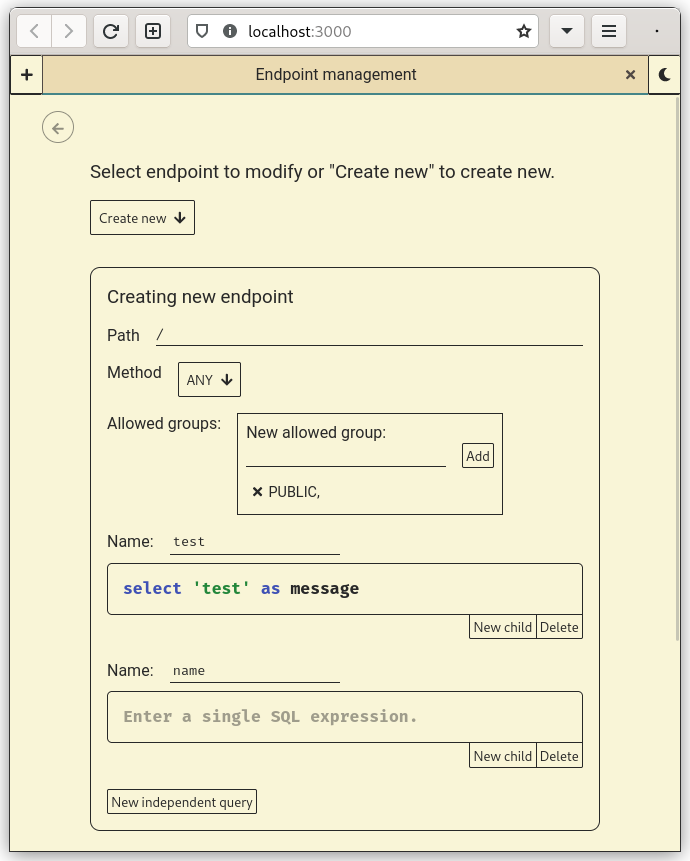
\includegraphics[width=.60\linewidth]{./img/endpoint_editor/creating_new/2.png} }}

                    \caption{Przebieg testu tworzenia nowego drzewa zapytań SQL}
                    \label{creatingNewTreeManualTest}
                \end{figure}

                \FloatBarrier

            \item \textbf{Testowanie poprawnego dodawania zapytania podrzędnego.}

                \textbf{Przebieg testu:}

                \begin{enumerate}

                    \item Wciśnięcie przycisku ``New child'' pod dowolnym polem
                        tekstowym z zapytaniem SQL.

                \end{enumerate}

                \textbf{Spodziewany wynik:}

                Pod zapytaniem zostanie dodane nowe zapytanie podrzędne do
                zapytania, którego przycisk wciśnięto. Zapytanie będzie
                posiadało większy margines z lewej strony. Zapytanie będzie
                znajdowało się po prawej stronie przedłużenia ramki pola
                tekstowego z zapytaniem nadrzędnym.

                Jeśli zapytanie, którego przycisk wciśnięto posiadało przycisk
                ``Delete'', przycisk ten zniknie i będzie widoczny ponownie
                dopiero, gdy zostaną usunięte wszystkie zapytania podrzędne do
                tego zapytania.

                Przebieg testu został przedstawiony na rysunku \ref{creatingNewSubTreeManualTest}.

                \begin{figure}[h]
                    \centering

                    \subfloat[\centering Przed wykonaniem]
                    {{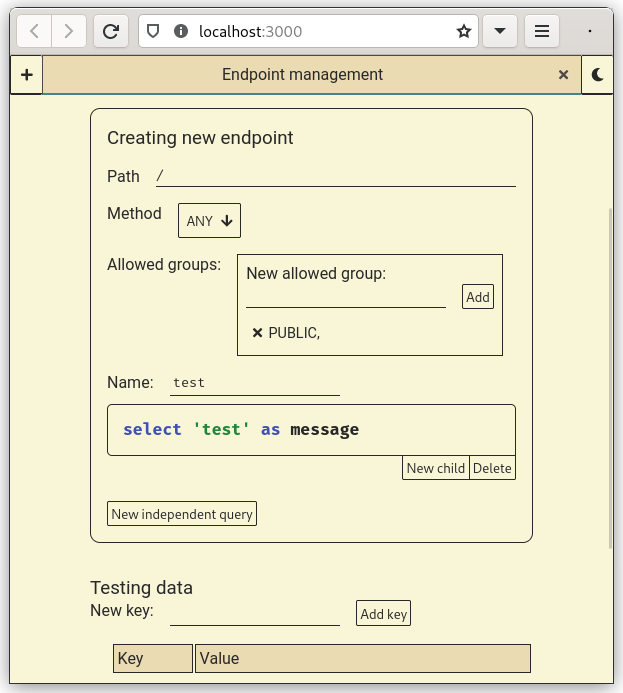
\includegraphics[width=.66\linewidth]{./img/endpoint_editor/creating_sub/1.png} }}

                    \subfloat[\centering Po wykonaniu]
                    {{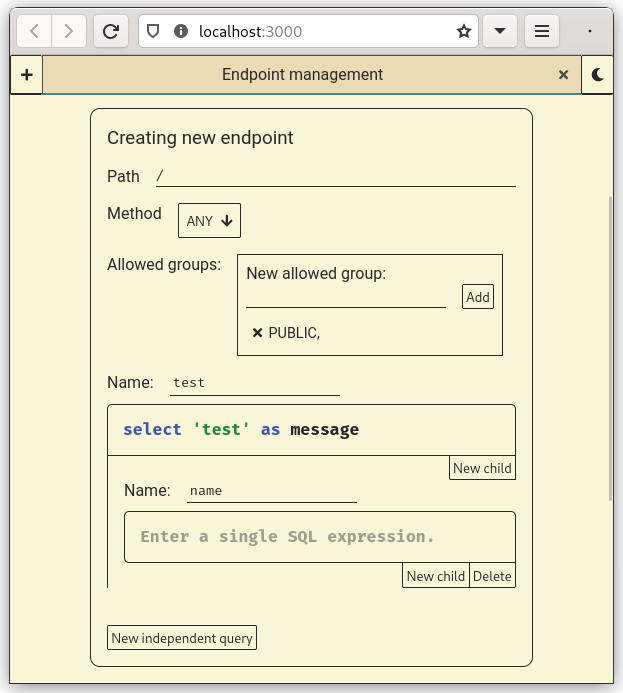
\includegraphics[width=.66\linewidth]{./img/endpoint_editor/creating_sub/2.png} }}

                    \caption{Przebieg testu tworzenia nowego podrzędnego drzewa zapytań SQL}
                    \label{creatingNewSubTreeManualTest}
                \end{figure}

                \FloatBarrier

            \item \textbf{Testowanie poprawnego usuwania zapytania SQL.}

                \textbf{Przebieg testu:}

                \begin{enumerate}

                    \item Wciśnięcie przycisku ``Delete'' pod dowolnym polem
                        tekstowym z zapytaniem SQL.

                \end{enumerate}

                \textbf{Spodziewany wynik:}

                Jeśli zapytanie było jedynym zapytaniem przypisanym do punktu
                końcowego i posiadało treść w polu tekstowym, treść pola
                testowego zostanie wykasowana.

                Jeśli zapytanie było jedynym zapytaniem przypisanym do punktu
                końcowego i nie posiadało treści w polu tekstowym, nic się nie
                stanie.

                Jeśli zapytanie nie było jedynym zapytaniem, całe pole tekstowe
                zostanie wykasowane.

                Przebieg testu został przedstawiony na rysunku \ref{deletingTreeManualTest}.

                \begin{figure}[h]
                    \centering

                    \subfloat[\centering Przed wykonaniem, gdy istnieje więcej, niż jedno drzewo]
                    {{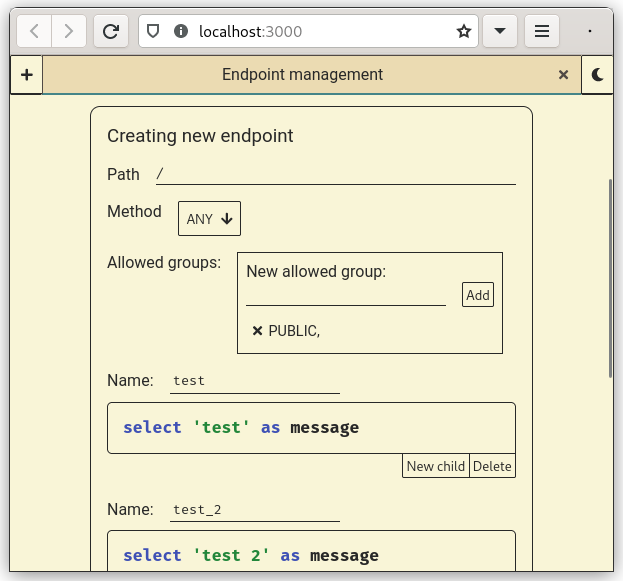
\includegraphics[width=.52\linewidth]{./img/endpoint_editor/deleting/1.png} }}
                    \medspace
                    \subfloat[\centering Po wykonaniu, gdy istniało więcej, niż jedno drzewo]
                    {{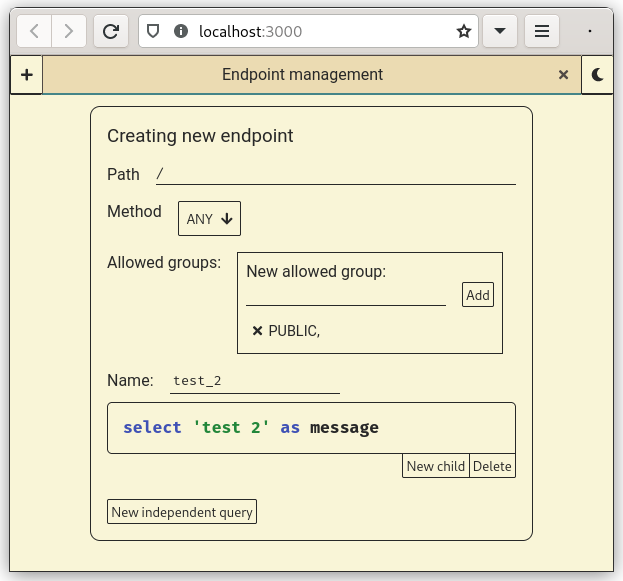
\includegraphics[width=.52\linewidth]{./img/endpoint_editor/deleting/2.png} }}

                    \subfloat[\centering Przed wykonaniem, gdy istnieje jedno drzewo]
                    {{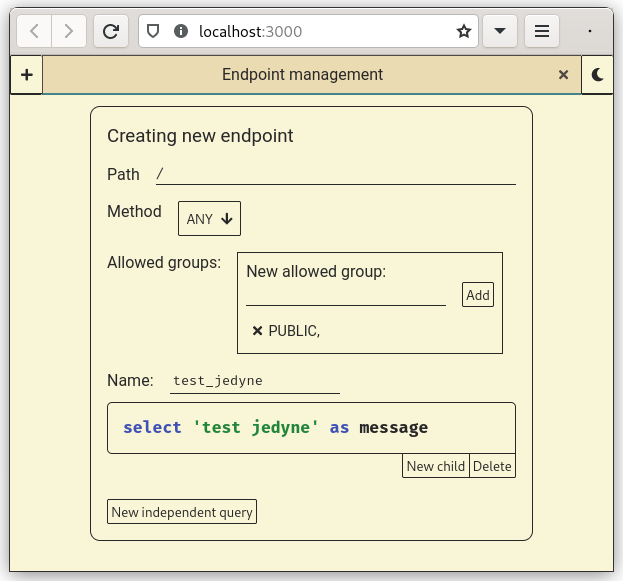
\includegraphics[width=.52\linewidth]{./img/endpoint_editor/deleting/3.png} }}
                    \medspace
                    \subfloat[\centering Po wykonaniu, gdy istniało jedno drzewo]
                    {{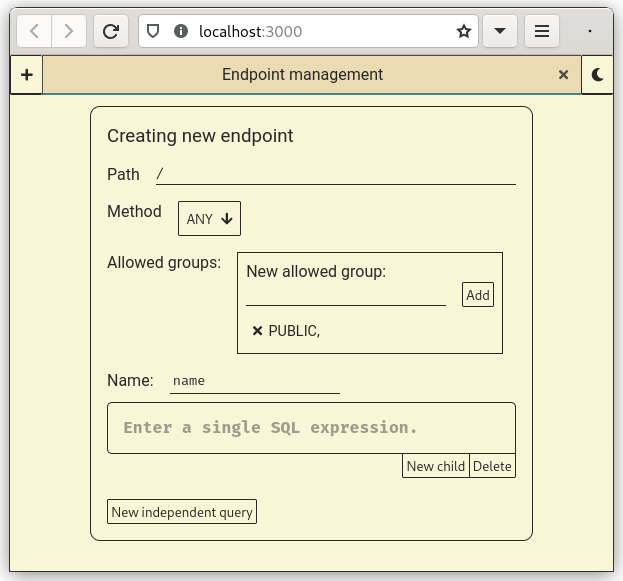
\includegraphics[width=.52\linewidth]{./img/endpoint_editor/deleting/4.png} }}

                    \caption{Przebieg testu usuwania drzewa zapytań SQL}
                    \label{deletingTreeManualTest}
                \end{figure}

                \FloatBarrier

            \item \textbf{Testowanie poprawnego dodawania nowego klucza do tabeli danych testowych
                pochodzących z zapytania.}

                \textbf{Przebieg testu:}

                \begin{enumerate}

                    \item Wpisanie dowolnej nazwy klucza w polu tekstowym ``New
                        key''.

                    \item Wciśnięcie przycisku ``Add key''.

                \end{enumerate}

                \textbf{Spodziewany wynik:}

                Do tabeli znajdującej się pod polem tekstowym zostanie dodany
                nowy rząd. W kolumnie ``Key'' znajdzie się klucz wpisany do pola
                tekstowego.

                Przebieg testu został przedstawiony na rysunku \ref{newTestDataKeyManualTest}.

                \begin{figure}[h]
                    \centering

                    \subfloat[\centering Przed wykonaniem]
                    {{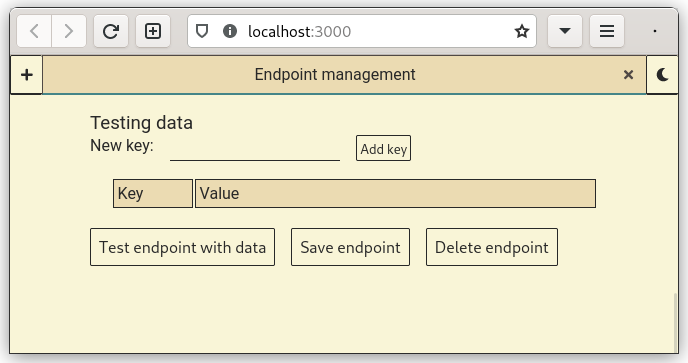
\includegraphics[width=.70\linewidth]{./img/endpoint_editor/test_data/1.png} }}

                    \subfloat[\centering Po wykonaniu]
                    {{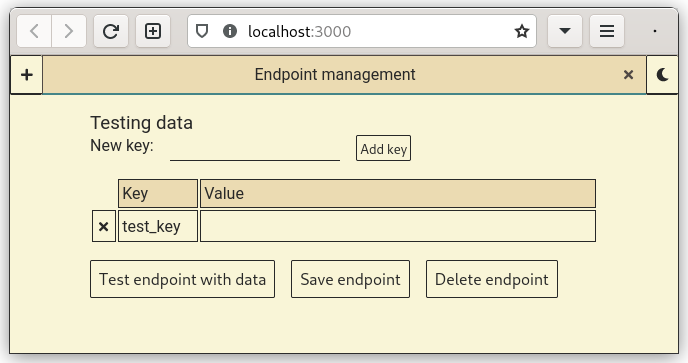
\includegraphics[width=.70\linewidth]{./img/endpoint_editor/test_data/2.png} }}

                    \caption{Przebieg testu dodawania nowego klucza do danych testowych}
                    \label{newTestDataKeyManualTest}
                \end{figure}

                \FloatBarrier

        \end{enumerate}

\end{enumerate}
